%----------------------------------------------------------------------------------------
%	PACKAGES AND OTHER DOCUMENT CONFIGURATIONS
%----------------------------------------------------------------------------------------

\documentclass[
		twoside,openright,titlepage,numbers=noenddot,headinclude,%1headlines,
	 	footinclude=true,cleardoublepage=empty,
		dottedtoc, % Make page numbers in the table of contents flushed right with dots leading to them
		BCOR=5mm,paper=a4,fontsize=11pt, % Binding correction, paper type and font size
		ngerman,american, % Languages, change this to your language(s)
		]{scrreprt} 
                
% Includes the file which contains all the document configurations and packages - make sure to edit this file

%----------------------------------------------------------------------------------------
%	CHARACTER ENCODING
%----------------------------------------------------------------------------------------

\PassOptionsToPackage{utf8}{inputenc} % Set the encoding of your files. UTF-8 is the only sensible encoding nowadays. If you can't read äöüßáéçèê∂åëæƒÏ€ then change the encoding setting in your editor, not the line below. If your editor does not support utf8 use another editor!
\usepackage{inputenc}

%----------------------------------------------------------------------------------------
%	DOCUMENT VARIABLES
%	Fill in the lines below to enter your information into the thesis template
%	Each of the commands can be cited anywhere in the thesis
%----------------------------------------------------------------------------------------

% Remove drafting to get rid of the '[ Date - classicthesis version 4.0 ]' text at the bottom of every page
\PassOptionsToPackage{eulerchapternumbers,listings,drafting, pdfspacing, subfig,beramono,eulermath,parts}{classicthesis}
% Available options: drafting parts nochapters linedheaders eulerchapternumbers beramono eulermath pdfspacing minionprospacing tocaligned dottedtoc manychapters listings floatperchapter subfig

\newcommand{\myTitle}{5C compliant low-level copter controller\xspace}
%\newcommand{\mySubtitle}{TODO subtitle\xspace}
\newcommand{\myDegree}{Automation Engineering\xspace}
\newcommand{\myName}{Federico Maria Rossi\xspace}
\newcommand{\myProf}{Prof. Lorenzo Marconi\xspace}
\newcommand{\myOtherProf}{Dr. Herman Bruyninckx\xspace}
\newcommand{\myFaculty}{Scuola di Ingegneria e Architettura\xspace}

\newcommand{\myLocation}{Bologna\xspace}
\newcommand{\myTimeCopyright}{2016-2017\xspace}
\newcommand{\myTime}{March 2017\xspace}
\newcommand{\myVersion}{version 1.2\xspace}

%----------------------------------------------------------------------------------------
%	USEFUL COMMANDS
%----------------------------------------------------------------------------------------

%\newcommand{\ie}{i.e.}
%\newcommand{\Ie}{I.e.}
%\newcommand{\eg}{e.g.}
%\newcommand{\Eg}{E.g.} 

\newcounter{dummy} % Necessary for correct hyperlinks (to index, bib, etc.)
\providecommand{\mLyX}{L\kern-.1667em\lower.25em\hbox{Y}\kern-.125emX\@}
\newlength{\abcd} % for ab..z string length calculation

%----------------------------------------------------------------------------------------
%	PACKAGES
%----------------------------------------------------------------------------------------

%\usepackage{lipsum} % Used for inserting dummy 'Lorem ipsum' text into the template

%------------------------------------------------

\PassOptionsToPackage{american}{babel}  % Change this to your language(s)
% Spanish languages need extra options in order to work with this template
%\PassOptionsToPackage{spanish,es-lcroman}{babel}
\usepackage{babel}

%------------------------------------------------			

\usepackage{csquotes}
\PassOptionsToPackage{%
%backend=biber, % Instead of bibtex
backend=bibtex8,bibencoding=ascii,%
language=auto,%
style=numeric-comp,%
%style=authoryear-comp, % Author 1999, 2010
%bibstyle=authoryear,dashed=false, % dashed: substitute rep. author with ---
sorting=nyt, % name, year, title
maxbibnames=10, % default: 3, et al.
%backref=true,%
natbib=true % natbib compatibility mode (\citep and \citet still work)
}{biblatex}
\usepackage{biblatex}
\addbibresource{Bibliography.bib}
 
 %------------------------------------------------

\PassOptionsToPackage{fleqn}{amsmath} % Math environments and more by the AMS 
 \usepackage{amsmath}
\PassOptionsToPackage{T1}{fontenc} % T2A for cyrillics
\usepackage{fontenc}
\usepackage{textcomp} % Fix warning with missing font shapes
\usepackage{scrhack} % Fix warnings when using KOMA with listings package  
\usepackage{xspace} % To get the spacing after macros right
\usepackage{mparhack} % To get marginpar right
\usepackage{fixltx2e} % Fixes some LaTeX stuff 
\PassOptionsToPackage{smaller}{acronym} % Include printonlyused in the first bracket to only show acronyms used in the text
\usepackage{acronym} % Nice macros for handling all acronyms in the thesis

%\renewcommand*{\acsfont}[1]{\textssc{#1}} % For MinionPro
\renewcommand*{\aclabelfont}[1]{\acsfont{#1}}
\PassOptionsToPackage{pdftex}{graphicx}
\usepackage{graphicx} 


\usepackage[rightcaption]{sidecap}
\graphicspath{ {gfx/} }
\usepackage{wrapfig}
%----------------------------------------------------------------------------------------
%	FLOATS: TABLES, FIGURES AND CAPTIONS SETUP
%----------------------------------------------------------------------------------------

\usepackage{tabularx} % Better tables
\setlength{\extrarowheight}{3pt} % Increase table row height
\newcommand{\tableheadline}[1]{\multicolumn{1}{c}{\spacedlowsmallcaps{#1}}}
\newcommand{\myfloatalign}{\centering} % To be used with each float for alignment
\usepackage{caption}
\captionsetup{font=small}
\usepackage{subfig}  

%----------------------------------------------------------------------------------------
%	CODE LISTINGS SETUP
%----------------------------------------------------------------------------------------

\usepackage{listings} 
%\lstset{emph={trueIndex,root},emphstyle=\color{BlueViolet}}%\underbar} % For special keywords
\lstset{language=[LaTeX]Tex,%C++ % Specify the language(s) for listings here
morekeywords={PassOptionsToPackage,selectlanguage},
keywordstyle=\color{RoyalBlue}, % Add \bfseries for bold
basicstyle=\small\ttfamily, % Makes listings a smaller font size and a different font
%identifierstyle=\color{NavyBlue}, % Color of text inside brackets
commentstyle=\color{Green}\ttfamily, % Color of comments
stringstyle=\rmfamily, % Font type to use for strings
numbers=left, % Change left to none to remove line numbers
numberstyle=\scriptsize, % Font size of the line numbers
stepnumber=5, % Increment of line numbers
numbersep=8pt, % Distance of line numbers from code listing
showstringspaces=false, % Sets whether spaces in strings should appear underlined
breaklines=true, % Force the code to stay in the confines of the listing box
%frameround=ftff, % Uncomment for rounded frame
%frame=single, % Frame border - none/leftline/topline/bottomline/lines/single/shadowbox/L
belowcaptionskip=.75\baselineskip % Space after the "Listing #: Desciption" text and the listing box
}

%----------------------------------------------------------------------------------------
%	HYPERREFERENCES
%----------------------------------------------------------------------------------------

\PassOptionsToPackage{pdftex,hyperfootnotes=false,pdfpagelabels}{hyperref}
\usepackage{hyperref}  % backref linktocpage pagebackref
\pdfcompresslevel=9
\pdfadjustspacing=1

\hypersetup{
% Uncomment the line below to remove all links (to references, figures, tables, etc), useful for b/w printouts
%draft, 
colorlinks=true, linktocpage=true, pdfstartpage=3, pdfstartview=FitV,
% Uncomment the line below if you want to have black links (e.g. for printing black and white)
%colorlinks=false, linktocpage=false, pdfborder={0 0 0}, pdfstartpage=3, pdfstartview=FitV, 
breaklinks=true, pdfpagemode=UseNone, pageanchor=true, pdfpagemode=UseOutlines,%
plainpages=false, bookmarksnumbered, bookmarksopen=true, bookmarksopenlevel=1,%
hypertexnames=true, pdfhighlight=/O,%nesting=true,%frenchlinks,%
urlcolor=webbrown, linkcolor=RoyalBlue, citecolor=webgreen, %pagecolor=RoyalBlue,%
    %urlcolor=Black, linkcolor=Black, citecolor=Black, %pagecolor=Black,%
%------------------------------------------------
% PDF file meta-information
pdftitle={\myTitle},
pdfauthor={\textcopyright\ \myName},
pdfsubject={},
pdfkeywords={},
pdfcreator={pdfLaTeX},
pdfproducer={LaTeX with hyperref and classicthesis}
%------------------------------------------------
}

%----------------------------------------------------------------------------------------
%	AUTOREFERENCES SETUP
%	Redefines how references in text are prefaced for different 
%	languages (e.g. "Section 1.2" or "section 1.2")
%----------------------------------------------------------------------------------------

\makeatletter
\@ifpackageloaded{babel}
{
\addto\extrasamerican{
\renewcommand*{\figureautorefname}{Figure}
\renewcommand*{\tableautorefname}{Table}
\renewcommand*{\partautorefname}{Part}
\renewcommand*{\chapterautorefname}{Chapter}
\renewcommand*{\sectionautorefname}{Section}
\renewcommand*{\subsectionautorefname}{Section}
\renewcommand*{\subsubsectionautorefname}{Section}
}
\addto\extrasngerman{
\renewcommand*{\paragraphautorefname}{Absatz}
\renewcommand*{\subparagraphautorefname}{Unterabsatz}
\renewcommand*{\footnoteautorefname}{Fu\"snote}
\renewcommand*{\FancyVerbLineautorefname}{Zeile}
\renewcommand*{\theoremautorefname}{Theorem}
\renewcommand*{\appendixautorefname}{Anhang}
\renewcommand*{\equationautorefname}{Gleichung}
\renewcommand*{\itemautorefname}{Punkt}
}
\providecommand{\subfigureautorefname}{\figureautorefname} % Fix to getting autorefs for subfigures right
}{\relax}
\makeatother

%----------------------------------------------------------------------------------------

\usepackage{classicthesis} 

%----------------------------------------------------------------------------------------
%	CHANGING TEXT AREA 
%----------------------------------------------------------------------------------------

%\linespread{1.05} % a bit more for Palatino
%\areaset[current]{312pt}{761pt} % 686 (factor 2.2) + 33 head + 42 head \the\footskip
%\setlength{\marginparwidth}{7em}%
%\setlength{\marginparsep}{2em}%

%----------------------------------------------------------------------------------------
%	USING DIFFERENT FONTS
%----------------------------------------------------------------------------------------

%\usepackage[oldstylenums]{kpfonts} % oldstyle notextcomp
%\usepackage[osf]{libertine}
%\usepackage[light,condensed,math]{iwona}
%\renewcommand{\sfdefault}{iwona}
%\usepackage{lmodern} % <-- no osf support :-(
%\usepackage{cfr-lm} % 
%\usepackage[urw-garamond]{mathdesign} <-- no osf support :-(
%\usepackage[default,osfigures]{opensans} % scale=0.95 
%\usepackage[sfdefault]{FiraSans}

\addbibresource{Bibliography.bib} % The file housing your bibliography
%\addbibresource[label=ownpubs]{Self_Publications.bib} % Uncomment for optional self-publications

%\hyphenation{Put special hyphenation here}
\DeclareMathAlphabet{\pazocal}{OMS}{zplm}{m}{n}
\usepackage{listings}

\lstset{basicstyle=\scriptsize\ttfamily,
	commentstyle=\ttfamily\itshape\color{gray},
	stringstyle=\ttfamily,
	showstringspaces=false,
	breaklines=true,
	frameround=ffff,
	frame=single,
	rulecolor=\color{black}
}
\usepackage{adjustbox}
\usepackage{blindtext}


\ifthenelse{\boolean{@drafting}}
{\renewcommand\myVersion{version 1.0\xspace}
	\renewcommand{\PrelimText}{%
		\footnotesize[\,\myTime\ -- \texttt{\myTitle}]}
	\renewcommand{\finalVersionString}{\emph{Final Version} as of \today\ (\texttt{\@title}~\myVersion).}
}



\begin{document}

\frenchspacing % Reduces space after periods to make text more compact

\raggedbottom % Makes all pages the height of the text on that page

\selectlanguage{american} % Select your default language - e.g. american or ngerman

%\renewcommand*{\bibname}{new name} % Uncomment to change the name of the bibliography
%\setbibpreamble{} % Uncomment to include a preamble to the bibliography - some text before the reference list starts

\pagenumbering{roman} % Roman page numbering prior to the start of the thesis content (i, ii, iii, etc)

\pagestyle{plain} % Suppress headers for the pre-content pages

%----------------------------------------------------------------------------------------
%	PRE-CONTENT THESIS PAGES
%----------------------------------------------------------------------------------------

% Title Page

\begin{titlepage}

\begin{addmargin}[-1cm]{-3cm}
\begin{center}
\large

\hfill


\textbf{{\Large ALMA MATER STUDIORUM - UNIVERSITÀ DI BOLOGNA\\}
}\noindent\makebox[\linewidth]{\rule{\textwidth}{0.4pt}}

{\Large \textbf{SCUOLA DI INGEGNERIA  E ARCHITETTURA\\}}

\vspace{1cm}

DIPARTIMENTO DI INGEGNERIA DELL'ENERGIA ELETTRICA E DELL'INFORMAZIONE\\

\vspace{1cm}

INGEGNERIA DELL'AUTOMAZIONE\\

\vspace{1cm}

{\Large \textbf{
TESI DI LAUREA\\
IN\\
ADVANCED CONTROL SYSTEMS M}}

\vspace{1cm}

\textbf{{\LARGE 5C COMPLIANT LOW-LEVEL COPTER CONTROLLER}}

\vfill{\Large 
\begin{tabular}{p{\textwidth}cc}
	\begin{tabular}{p{\textwidth}c}
		Candidato:\\
		Federico Maria Rossi
	\end{tabular}
	&
	\begin{tabular}{p{\textwidth}c}
		Relatore:\\
		Prof. Lorenzo Marconi
	\end{tabular}
\end{tabular}}

\vfill


Anno Accademico 2016/17

Sessione III

\vfill

\end{center}
\end{addmargin}

\end{titlepage} % Main title page
% Back of the title page

\thispagestyle{empty}

\hfill

\vfill

\noindent\myName: \textit{\myTitle} %\myDegree, 
\textcopyright\ \myTime

% You may wish to do something with the back of the title page, such as including your supervisors, location or time frame of the work. Below is an example of doing so although you may want to tweak it to your liking.

\bigskip

\noindent\spacedlowsmallcaps{Supervisors}: \\
\myProf \\
\myOtherProf \\ 
%\mySupervisor

%\medskip \\

%\noindent\spacedlowsmallcaps{Location}: \\
%\myLocation

%\medskip \\

%\noindent\spacedlowsmallcaps{Time Frame}: \\
%\myTime
 % Back of the title page
%\cleardoublepage% Dedication

\thispagestyle{empty}
\refstepcounter{dummy}

\pdfbookmark[1]{Dedication}{Dedication} % Bookmark name visible in a PDF viewer

\vspace*{3cm}

\begin{center}
\emph{Ohana} means family. \\
Family means nobody gets left behind, or forgotten. \\ \medskip
--- Lilo \& Stitch    
\end{center}

\medskip

\begin{center}
Dedicated to the loving memory of Rudolf Miede. \\ \smallskip
1939\,--\,2005
\end{center} % Dedication page
%\cleardoublepage\include{FrontBackMatter/Foreword} % Uncomment and create a Foreword.tex to include a foreword
\cleardoublepage% Abstract

%\renewcommand{\abstractname}{Abstract} % Uncomment to change the name of the abstract

\pdfbookmark[1]{Abstract}{Abstract} % Bookmark name visible in a PDF viewer

\begingroup
\let\clearpage\relax
\let\cleardoublepage\relax
\let\cleardoublepage\relax

\chapter*{Abstract}
Modern engineering faces the problem of implementing systems in a flexible, scalable and reusable way. This problem becomes exponentially hard as the complexity of systems increase, unless systems and systems components developers foresees and find ways to overcome such scaling problematic.

Many techniques try to address the scaling problem by defining paradigms to standardize or, at least, harmonize the efforts of different developers teams. Nevertheless developers tends to underestimate their importance, either because of lack of education, either because they consider overcomplicated or pointless their adoption in small to medium projects. This is indeed true sometimes: the lack of mature, open, free, supported and widely accepted tools makes the benefit one can archive from the introduction of such techniques void w.r.t. the effort required to learn and adopt them. This is a vicious cycle, however projects like ROS
\graffito{ROS is a open-source component based software framework, where components are usually written and released by third party developers for being reused, avoiding the necessity of "re-inventing the wheel"}
show how also small projects can benefit from a proper and formal approach to the problem, especially once a "critical mass" of adopters is reached.

This thesis provides a study case: the Model Driven Engineering (MDE) methodology and the 5C "separation of software behavior" paradigm are applied in the development of a novel low-level copter controller. The following chapters will briefly introduce such techniques and will show how to apply them in a real-world problem.
\\
\\
As already highlighted, such small and stand-alone application does not gain enough benefit from this approach to justify the effort required, however the purpose of this thesis is to support and popularize a certain attitude to problems approach, to release working example code, contribute to the maturity of the underlying software framework and, last but not least, to enrich the knowledge and the skills of author readers.

\endgroup			

\vfill % Abstract page
%\cleardoublepage% Publications - a page listing research articles written using content in the thesis

\pdfbookmark[1]{Publications}{Publications} % Bookmark name visible in a PDF viewer

\chapter*{Publications} % Publications page text

Some ideas and figures have appeared previously in the following publications:\\

\noindent Put your publications from the thesis here. The packages \texttt{multibib} or \texttt{bibtopic} etc. can be used to handle multiple different bibliographies in your document.

%\begin{refsection}[ownpubs]
%    \small
%    \nocite{*} % is local to to the enclosing refsection
%    \printbibliography[heading=none]
%\end{refsection}

%\emph{Attention}: This requires a separate run of \texttt{bibtex} for your \texttt{refsection}, \eg, \texttt{ClassicThesis1-blx} for this file. You might also use \texttt{biber} as the backend for \texttt{biblatex}. See also \url{http://tex.stackexchange.com/questions/128196/problem-with-refsection}. % Publications from the thesis page
\cleardoublepage% Acknowledgements

\pdfbookmark[1]{Acknowledgements}{Acknowledgements} % Bookmark name visible in a PDF viewer

\begin{flushright}{\slshape    
We have seen that computer programming is an art, \\ 
because it applies accumulated knowledge to the world, \\ 
because it requires skill and ingenuity, and especially \\
because it produces objects of beauty.} \\ \medskip
--- {Donald E. Knuth}
\end{flushright}

\bigskip

%----------------------------------------------------------------------------------------

\begingroup

\let\clearpage\relax
\let\cleardoublepage\relax
\let\cleardoublepage\relax

\chapter{Acknowledgements}

First and foremost I want to thank my family for all their love and encouragement. For my parents who raised me with a love of science and supported me in all my pursuits.\\
I am grateful to my supervisor Prof. Lorenzo Marconi that helped me in my thesis and to my co-supervisor Dr. Herman Bruyninckx that really opened my mind.\\
Thanks to the whole ROB group, especially Nico Huebel, Enea Scioni and Lin Zhang for their support and their company during my work.

\endgroup % Acknowledgements page
\pagestyle{scrheadings} % Show chapter titles as headings
%\cleardoublepage% Table of Contents - List of Tables/Figures/Listings and Acronyms

\refstepcounter{dummy}

\pdfbookmark[1]{\contentsname}{tableofcontents} % Bookmark name visible in a PDF viewer

\setcounter{tocdepth}{2} % Depth of sections to include in the table of contents - currently up to subsections

\setcounter{secnumdepth}{3} % Depth of sections to number in the text itself - currently up to subsubsections

\manualmark
\markboth{\spacedlowsmallcaps{\contentsname}}{\spacedlowsmallcaps{\contentsname}}
\tableofcontents 
\automark[section]{chapter}
\renewcommand{\chaptermark}[1]{\markboth{\spacedlowsmallcaps{#1}}{\spacedlowsmallcaps{#1}}}
\renewcommand{\sectionmark}[1]{\markright{\thesection\enspace\spacedlowsmallcaps{#1}}}

\clearpage

\begingroup 
\let\clearpage\relax
\let\cleardoublepage\relax
\let\cleardoublepage\relax

%----------------------------------------------------------------------------------------
%	List of Figures
%----------------------------------------------------------------------------------------

%\refstepcounter{dummy}
%\addcontentsline{toc}{chapter}{\listfigurename} % Uncomment if you would like the list of figures to appear in the table of contents
%\pdfbookmark[1]{\listfigurename}{lof} % Bookmark name visible in a PDF viewer

%\listoffigures

\vspace{8ex}
\newpage

%----------------------------------------------------------------------------------------
%	List of Tables
%----------------------------------------------------------------------------------------

%\refstepcounter{dummy}
%\addcontentsline{toc}{chapter}{\listtablename} % Uncomment if you would like the list of tables to appear in the table of contents
%\pdfbookmark[1]{\listtablename}{lot} % Bookmark name visible in a PDF viewer

%\listoftables
        
\vspace{8ex}
\newpage
    
%----------------------------------------------------------------------------------------
%	List of Listings
%---------------------------------------------------------------------------------------- 

\refstepcounter{dummy}
%\addcontentsline{toc}{chapter}{\lstlistlistingname} % Uncomment if you would like the list of listings to appear in the table of contents
\pdfbookmark[1]{\lstlistlistingname}{lol} % Bookmark name visible in a PDF viewer

\lstlistoflistings 

\vspace{8ex}
\newpage
       
%----------------------------------------------------------------------------------------
%	Acronyms
%----------------------------------------------------------------------------------------

%\refstepcounter{dummy}
%\addcontentsline{toc}{chapter}{Acronyms} % Uncomment if you would like the acronyms to appear in the table of contents
%\pdfbookmark[1]{Acronyms}{acronyms} % Bookmark name visible in a PDF viewer

%\markboth{\spacedlowsmallcaps{Acronyms}}{\spacedlowsmallcaps{Acronyms}}

%\chapter*{Acronyms}

%\begin{acronym}[UML]
%\acro{DRY}{Don't Repeat Yourself}
%\acro{API}{Application Programming Interface}
%\acro{UML}{Unified Modeling Language}
%\end{acronym}  
                   
\endgroup % Contents, list of figures/tables/listings and acronyms
%\cleardoublepage
\pagenumbering{arabic} % Arabic page numbering for thesis content (1, 2, 3, etc)
%\setcounter{page}{90} % Uncomment to manually start the page counter at an arbitrary value (for example if you wish to count the pre-content pages in the page count)
\cleardoublepage % Avoids problems with pdfbookmark

%----------------------------------------------------------------------------------------
%	THESIS CONTENT - CHAPTERS
%----------------------------------------------------------------------------------------


\part{Background}
\chapter{Introduction}
\label{ch:introduction} 
Every day new technologies are available on the market making the realization of advanced robotics applications easier and accessible to large public. This is leading to a spread of a  number of different approaches to typical problems causing many redundant implementations of relatively common problems and, usually, waste of energy.\\
This thesis investigates a flexible and scalable approach to the development of software for robotics, trying to maximize the potentiality of the underlying components while abstracting the complexity of the low-level implementation. The software has been implemented on a new component-based software framework, trying to surmount the limits of other (sometimes more mature) frameworks like Open-RTM, ROS, OPRoS and SmartSoft.\\
\\
Details on this work will be explained in the details in this thesis; the sources of the software and everything necessary to reproduce the results can be found in the following git repositories.
\begin{itemize}
	\item The LaTeX source of this thesis:\\
	\texttt{https://github.com/fmr42/MasterThesis}\\
	
	\item The UBX project forked from the original repo to support system-wide installation:\\
	\texttt{https://bitbucket.org/fmr42/ubx-core/}\\
	\texttt{https://bitbucket.org/fmr42/ubx-base/}\\
	
	\item The controller here presented and the \texttt{bcsk} library it depends on:\\
	\texttt{https://github.com/fmr42/bcsk}\\
	\texttt{https://bitbucket.org/fmr42/ubx-control/}\\
\end{itemize}

This software has been developed and tested on a Fedora 21 GNU/Linux system running on AMD64 processor and on an Ubuntu Trusty 14.04 running on an ARM processor, however everything as been studied to be highly portable and, once satisfied the dependencies, should compile an all POSIX-compliant platform (Linux, OSX, BSD). % Chapter 1
\cleardoublepage % Empty page before the start of the next part

%------------------------------------------------

\chapter{Model driven engineering}
\label{ch:mdl}
Model driven engineering (MDE from now on) is a promising approach to problem solving, especially in complex applications. MDE alleviate the complexity of the problem by using a domain specific language to express domain specific concepts. This aims to maximize compatibility between systems, especially those implemented by different individuals or different teams: such goal is archived by making terminology and design patterns uniform.
While MDE is quite popular in software engineering (especially in large software projects), it is still considered not necessary in fields like robotics where the

\section{Metamodelling}
A model is an abstraction of a real system and it exactly describes its behavior; multiple systems can conform to the same model, meaning that they behave the same (e.g. multiple implementations of a control system).
The same way, a meta-model is a model of models, meaning that it is yet another abstraction; it is used to describe at a more conceptual level rules and constraints of a given class of models. To make an example, in the study case presented in this thesis the extended Kalman filter conforms to the mathematical model of an extended Kalman filter which in turns conforms to the meta-model of a \emph{state estimator} like models of other types of filters, e.g. a particle filter.

\section{Domain specific languages}
Domain specific languages (DSL) are languages specifically designed to easily express schemes or patterns commons within a certain field, without the need of details of some particular implementation. DSL are commonly used to describe models and meta-models.

 % Chapter 1
\cleardoublepage % Empty page before the start of the next part

%------------------------------------------------

\chapter{Approach to the problem}
\label{ch:sense-plan-act}
In the following two different control strategy are compared: the \emph{sense-plan-act} and the \emph{task-skill-motion} strategy. Pro and cons of the two approaches are compared to justify the choices made within this thesis.

\section{Sense-plan-act}
\graffito{Although this may seems the fastest and simpler approach, on a long-term period causes many redundant and bug-prone re-implementation of the same patterns.}A common approach to control is to solve the overall complex problem by combining the low-level functionalities of the underlying platform into a monolithic control loop, resulting in a controller strictly tied to that specific problem and therefore poorly re-usable\graffito{Sometimes it is more convenient to re-implement from scratch then re-use old (maybe well-tested!) solutions...}.\\
From a long-term prospective, it is wider to spend more time during the development to come out with a scalable solution for the future.

\section{Task-skill-motion}
Although sense-plan-act is the most widely used control strategy, other alternatives have been proposed. As in MDE we use different DSL's to represent the behavior of the system to be controlled at different levels of abstraction, we can in the same way define multiple control loops, one for every level of behavior abstraction. In many complex application it is usually present a mission composed by more task. Each task can be realized employing the skills of the platform and each skill if archived by low-level motion control.\\
\begin{wrapfigure}{r}{0.5\textwidth} %this figure will be at the right
	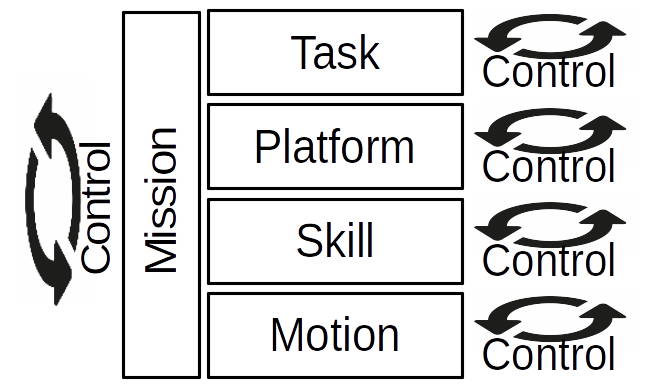
\includegraphics[width=0.7\textwidth]{taskSkillMotion}
	\caption{The task-skill-motion control strategy.}
	\label{fig:taskSkillMotion}
\end{wrapfigure}
We can see that the mission is a far more abstract control problem than the low-level actuation: a mission can be coordinated by a software or human supervisor, usually with more relaxed time constraints, and may distribute the necessary tasks to more agents. Each agent may than decide how to complete the task autonomously, on the basis of its own skills (which obviously depend on the actual hardware platform on which the agent is running). In turn, the skills are composed by one or more low-level motions.\\
The control problem proposed in this thesis implements a skill (i.e. the ability of the vehicle to fly around) by combining motions (that are the actual control inputs to the actuators). This skill is actually controlled by a human interface but everything has been studied to integrate the solution to such context.
 % Chapter 1
\cleardoublepage % Empty page before the start of the next part

%------------------------------------------------

\chapter{The 5C's of robotics}

\label{ch:introduction} 
\section{50 years of }
Most engineering problems are still solved as particular and stand-alone problems, so if a solution is not already available for that problem, a new one is developed with no concerns of making that solution re-usable for similar problems. Industrial research often force the researchers to opt for a quick, simple and cost-effective solution, ignoring the fact that tens or hundreds (maybe thousands!) of other engineers already addressed that problem, re-implementing the solution almost each time. Certainly it would be useful to reuse the same solution if possible, eventually improving it if it does not exactly fit the problem.
\section{Separation of concerns}
The separation of concerns if an approach to the code re usability problem promoted by BRICS. Researchers had identified 4 possible concerns, or behavior, that should be kept distinct with the goal of decoupling them and allowing an easy and standardized practice to re-use them across different applications, but also to make it easy to re-implement or substitute them within the \emph{same} application. These behaviors are computation, communication, coordination and configuration\cite{brics}.
\begin{wrapfigure}{r}{0.25\textwidth} %this figure will be at the right
	\label{fig:fivec}
	\centering
	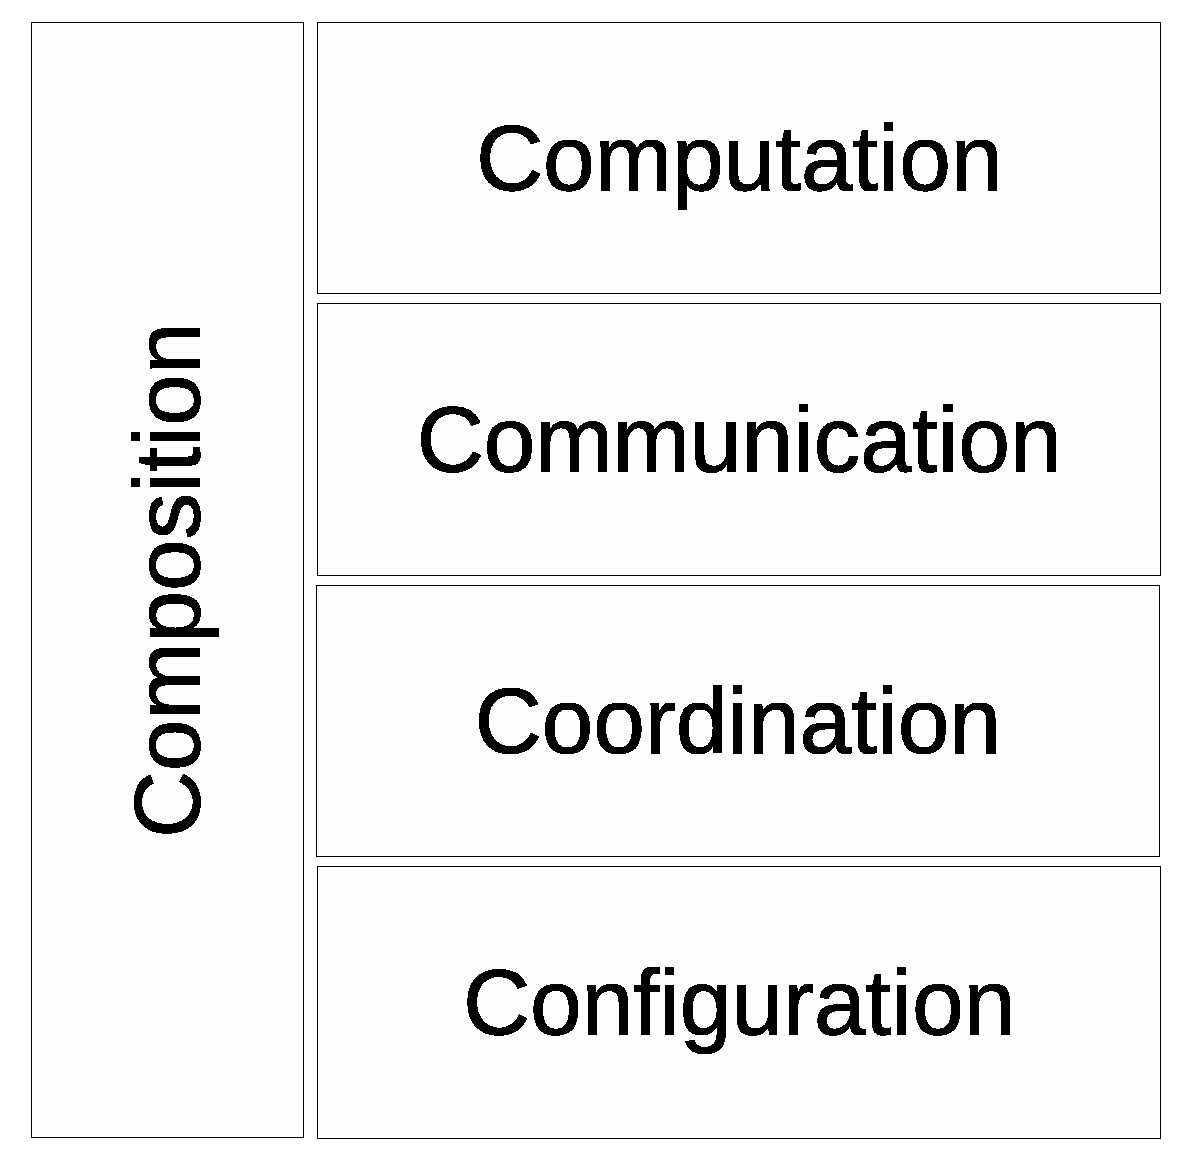
\includegraphics[width=0.5\textwidth]{5c}
%	The 4 behaviors of a system, glued by the composability property.
%		\label{fig:5c}
%		\ref{fig:5c}
\end{wrapfigure}
An additional concern was added to give this practice a good trade-off between scalability and complexity: more components can be composed to obtain a new component also having only one of the listed possible behaviors.
\subsection{Computation}
Computation is the core of a system functionality: it usually require read and/or write access to data, configuration and synchronization to produce the expected result.
\subsection{Communication}
Communication is responsible for data transmission between different computational components with the proper quality of service. A communication component usually store and retrieve data for computational components. In case a communication block do actually communicate with \emph{other} agents, it is named a \emph{bridge}.
\subsection{Coordination}
Coordination is responsible for the actual discrete behavior of the system and can be represented by a finite state machine, in other words it ensures the correct computational behavior at the correct time.
\subsection{Configuration}
Configuration is also responsible for the behavior of single computation or communication components; should be kept distinct and, indeed, configurable. Bad practice in software engineering is to hard-code configuration values; yet there are obvious exceptions like mathematical constants, e.g. $\pi$.
\subsection{Composition}
While separation of the previous 4 concerns gives a way to de-couple a system components, it is still necessary to introduce a trade-off between modularity and simplicity of the implementation. For this reason the last introduced behavior is \emph{composition} which gives the capability of combining components (with different concerns) into a macro component which in turn has one of the described behavior.




 % Chapter 1
\cleardoublepage % Empty page before the start of the next part

%------------------------------------------------

\part{The study case}
\chapter{The control algorithm}
\label{ch:controlalgorithm} 
Unmanned aerial vehicles (UAVs) are a class of aircraft under the control of either a remote human pilot or a on board computer. UAVs were originally developed for military purposes, although recent advances in technologies, like Li-Ion batteries and brush-less motors, have brought this type of aircraft to  others scopes of usage, like commercial, scientific and also recreational.
Although most UAVs are fixed-wing aircraft, rotorcraft are becoming popular too due to the low price and ease of maintenance and run.\graffito{Quad-copter, more commonly referred to as \emph{drones}, are commercially available to a large amateur public.} The demand for this type of drone is increasing and the global market for commercial use is expected to grow in the next few years, thats why the study case is a low-level controller for helicopters, ducted-fan tail-sitters and multi-propeller helicopters.

\section{A novel approach to the copter control proble}
A common control strategy is a cascade feedback: an outer loop for the position and an inner loop for the attitude. The inner control loop is usually composed by 3 control loop for the roll, pitch and yaw attitude angles. While this is a easy and intuitive approach to the problem, a more advanced one can be developed: the rest of this chapter describes a novel approach as presented in \autocite{marconi}.

\section{Quaternions for rotations representation}
Although the attitude has 3 degrees of freedom\graffito{Rotations of 3D objects in a 3D world can be expressed by 3 scalar quantities, usually Euler angles or roll-pitch-yaw angles (RPY).}, any minimal parametrization suffers of singularity problems (or gimbals-look).\\
\graffito{A rotation matrix is a 3x3 orto-normal matrix, so although it is composed by 9 scalar values, the matrix itself has just 3 degrees of freedom}
A very common alternative representation is rotational matrices: those do not suffer of singularities problems but are quite  redundant since 9 scalar values are used to express just 3 degrees of freedom.\\
A good trade-off between compactness and ease of representation is archived with unit quaternions, a notation that allows to represent rotations in a compact form and with no gimbals-lock problems. Another advantage to consider is numerical stability: numerical drifts make both rotation matrices and unit quaternions loose their own properties: respectively being orthonormal and having module one; it is however way easier to scale a vector than force the orthonormal structure of a matrix. More details can be found in \cite{bib:quat} and \cite{bib:rotquat}.\\
No insight in Hamiltonian math is reported there, it just follows a note about the notation used in the following chapters: in general a quaternion $q$ is given by:
\begin{equation} \label{eq:coptermodelmat}
\begin{split}
q := \begin{bmatrix}
\eta\\
\epsilon
\end{bmatrix}
\end{split}
\end{equation}
where $\eta$ is the \emph{real} component and $\epsilon$ is the \emph{pure imaginary} vector component of $q$ and the Hamilton product between 2 quaternion is indicated by the symbol $\oplus$.

\section{The copter model}
The dynamic model of the copter is given by:

\begin{equation} \label{eq:coptermodelmat}
\begin{split}
	M \ddot{p} &= -u_{f}Re_{3} + Mge_{3}\\
	\dot{R} &= RS(w)\\
	J\dot{w} &= S (Jw) w + u_{\tau}
\end{split}
\end{equation}

Where we call $ p $ the position vector of the center of gravity of the copter in the inertial reference frame $ \pazocal{F}_{i} $ and $ w $ the angular velocity of the vehicle in the body reference frame $ \pazocal{F}_{b} $. $ R $ is the rotation matrix representing the orientation of $ \pazocal{F}_{b} $ wrt $ \pazocal{F}_{i} $, $ J $ is the inertia matrix of the system and $ u_{f} $ and $ u_{\tau} $ are respectively the force and  the torque vector generated by the propellers.\graffito{Note that the while the $u_{f}$ is a scalar force which direction always aligned with the $z$ axis of $\pazocal{F}_{b}$, $u_{\tau}$ is a 3-dimensional vector.}
The $S(m)$ function generates a $3\times3$ matrix from vector $m$ such that the matrix product between $S(m)$ and another $3\times1$ vector $n$ correspond to the cross (vector) product between $m$ and $n$. $S$ can be constructed as:
\begin{equation} \label{eq:coptermodelmat}
\begin{split}
S(m) :&= \begin{bmatrix}
0 & -m_{3} & m_{2}\\
m_{3} & 0 & -m_{1}\\
-m_{2} & m_{1} & 0
\end{bmatrix}
\end{split}
\end{equation}

The copter model can be rewritten using quaternions to represent rotations by mean of the Rodriguez formula\cite{bib:rodriguez}:
\[ \pazocal{R}(q) = I + 2 \mu \pazocal{S}(\epsilon) + 2 \pazocal{S}(\epsilon)^{2}
 \]
as
\begin{equation} \label{eq:coptermodelquat}
\begin{split}
M \ddot{p} &= -u_{f}\pazocal{R}(q)e_{3} + Mge_{3}\\
\dot{q} &= \frac{1}{2} q \oplus \begin{bmatrix} 0 \\ w \end{bmatrix} \\
J\dot{w} &= S (Jw) w + u_{\tau}
\end{split}
\end{equation}



\section{Position control loop}
We can write the position error dynamic as:
\begin{equation} \label{eq:poserrdyn}
\begin{split}
M \ddot{\overline{p}} &= -u_{f}\pazocal{R}e_{3} + Mge_{3} - M\ddot{p}_{R}
\end{split}
\end{equation}
And define the control force as:
\begin{equation} \label{eq:ctrlforce}
\begin{split}
v^{c}_{R}(\ddot{p}_{R})&:=Mge_{3} - M\ddot{p}_{R}\\
v^{c}(\overline{p},\dot{\overline{p}},\ddot{p}_{R})&:=v^{c}_{R}(\ddot{p}_{R}) + \kappa(\overline{p},\dot{\overline{p}} )
\end{split}
\end{equation}
where $ \kappa(\overline{p},\dot{\overline{p}}) $ is a feedback action that can be computed as follow:
\begin{equation} \label{eq:feedback}
\begin{split}
\zeta_{1}&:=\overline{p}\\
\zeta_{2}&=\dot{\overline{p}} + \lambda_{1} \sigma (\frac{k_{1}}{\lambda_{1}}\lambda_{2})\\
\kappa(\overline{p},\dot{\overline{p}}) &:=\lambda_{2}\sigma(\frac{k_{2}}{\lambda{2}}\zeta_{2})
\end{split}
\end{equation}
where $k_{1}$, $k_{2}$, $\lambda_{1}$ and $\lambda_{2}$ are parameters to be tuned.\\
In \autoref{eq:ctrlforce} is mandatory to respect the constraint
\begin{equation} \label{eq:const}
\begin{split}
R_{R}e_{3} &= \frac{v^{c}_{R}(\ddot{p}_{R})}{\lVert v^{c}_{R}(\ddot{p}_{R})\rVert}
\end{split}
\end{equation}

The control scalar control force is than computed as:
\begin{equation} \label{eq:controlForce}
\begin{split}
u_{f} &:= \lVert v^{c}(\overline{p},\dot{\overline{p}},\ddot{p}_{R})\rVert
\end{split}
\end{equation}
\autoref{eq:controlForce} gives the total thrust the propeller should generate, however as already explained it is also necessary to compute the torque necessary to correct the vehicle attitude.\\
\autoref{sec:attControlLoop} will describe the attitude control low.

\section{Attitude control loop}\label{sec:attControlLoop}
The torque control vector is computed in a control loop nested into the position control loop, therefore, as usual in cascade control loops, it has a faster dynamic.
We start by defining the error attitude quaternion and the error angular velocity vector:
\begin{equation} \label{eq:qerr}
\begin{split}
\overline{q}&=q_{c}^{-1}\oplus q\\
\overline{w}:&=w-\overline{w}_{c}\\
\end{split}
\end{equation}
with
\begin{equation}
\begin{split}
\overline{w}_{c}:&=\pazocal{R}(\overline{q})^{T}w_{c}
\end{split}
\end{equation}
and $q_{c}$ computed as explained in \autoref{se:attSP}.

Then the control torque is given by:
\begin{equation}
\begin{split}
u_{\tau}&=u_{\tau}^{FF}(\overline{q},w_{c},\dot{w}_{c})   + u_{\tau}^{FB}(\overline{q},\overline{w},\overline{h})\\
u_{\tau}^{FF}(\overline{q},w_{c},\dot{w}_{c})   &=  J\pazocal{R}(\overline{q})^{T}\dot{w}_{c}   - S(J\overline{w}_{c}) \overline{w}_{c}\\
u_{\tau}^{FB}(\overline{q},\overline{w},\overline{h})   &=  -k_{p}\overline{h}\overline{\epsilon}  -k_{d}\overline{w}
\end{split}
\end{equation}
In the previous formula $k_{p}$ and $k_{d}$ are positive gains and $\overline{h} = \{-1,1\}$ is obtained by the hybrid function $\pazocal{H}_{c}$
\begin{equation}
\begin{split}
\pazocal{H}_{c} &= \begin{cases} \dot{\overline{h}} = 0  & \overline{h}\overline{\eta} \geq -\delta \\ \overline{h}^{+} \in \overline{sgn}(\overline{\eta}) & \overline{h}\overline{\eta} \leq -\delta  \end{cases}\\
\overline{sgn}(s) &= \begin{cases} sgn(s)  & \lvert s \rvert > 0 \\ \{-1,1\} &  s=0 \end{cases}\\
\end{split}
\end{equation}
$\eta \in (0,1)$ is the hysteresis threshold.\\

The control problem is more extensively explained in \autocite{marconi}, however the article does not specify how to compute the reference attitude $R_{R}$; this problem is addressed in the following section.


\section{Attitude set-point generation} \label{se:attSP}
The attitude reference orientation should be computed satisfying constraint \ref{eq:const}. The problem has just 1 degree of freedom which, for standard uses cases (i.e. for non acrobatic maneuver), is the vehicle yaw angle.\\
This thesis proposes an algorithm to compute the reference rotation matrix $R_{R}$ based on geometric projection. Considering the $yaw$ angle given, then the heading vector is defined as:
\begin{equation}
\begin{split}
d(yaw) &= [\cos{(yaw)} , \sin{(yaw)} , 0]^{T}
\end{split}
\end{equation}
The matrix $R_{R}$ is computed column-by-column as follows:
\begin{equation}
\begin{split}
R_{R}e_{3} :&= \frac{g e_{3} - \ddot{p}}{\lVert g e_{3} - \ddot{p} \rVert}\\
R_{R}e_{2} :&= \frac{R_{R}e_{3} \times d(yaw)}{\lVert R_{R}e_{3} \times d(yaw)  \rVert}\\
R_{R}e_{1} :&= \frac{R_{R}e_{2} \times R_{R}e_{3}}{\lVert R_{R}e_{2} \times R_{R}e_{3} \rVert}
\end{split}
\end{equation}
This technique allows to easily compute the reference rotation matrix that can be then easily converted to the quaternion rotation thanks to the Rodriguez formula.
The control attitude required in \autoref{eq:qerr} is then computed as follows:
\begin{equation}
\begin{split}
R_{c}e_{3} :&= \frac{v_{c} }{\lVert v_{c}  \rVert} \\
R_{c}e_{1} :&= \frac{R_{R}e_{1} \times R_{c}e_{3}}{\lVert R_{R}e_{1} \times R_{c}e_{3} \rVert}  \\
R_{c}e_{2} :&= \frac{R_{c}e_{3} \times R_{c}e_{1}}{\lVert R_{c}e_{3} \times R_{c}e_{1} \rVert}  
\end{split}
\end{equation}
end finally
\begin{equation}
\begin{split}
q_{c} &= \pazocal{R}^{-1}(R_{c})
\end{split}
\end{equation}
 % Chapter 2
\cleardoublepage % Empty page before the start of the next part

%------------------------------------------------

\chapter{UBX Framework}
\label{ch:introduction} 
UBX is a novel framework created to support the development of 5C compliant programs. The coder does not have to write and compile an executable (indeed, the \emph{behaviors} of the implemented algorithm should be kept isolated) but have to write and compile special \emph{function blocks} which in turns implements those behaviors and are then composed \emph{at runtime} by UBX to produce the desired result. Blocks are actually nothing more than functions contained in libraries, the path of those libraries and how the ports of the blocks should be connected is specified in a configuration file. 

\subsection{Environment}
A UBX program instance is named \emph{node}. A node is a set of blocks properly connected. There are 3 types of blocks:

\begin{itemize}
	\item i-blocks: those blocks are capable of storing, transmitting and/or receiving data; they implement the communication and configuration behavior of the node (therefore i-blocks should not manipulate data); they only have an input port (to which data can be written) and an output port (from wich data can be read); i-blocks capable of communications out of the scope of the node are named \emph{bridges};
	\item c-blocks: are responsible for the computational behavior of the node; when triggered, they can read and/or write from/to i-blocks and perform calculus; c-blocks can have an arbitrary number of input/output ports and must have a trigger port;
	\item s-blocks: implement the coordination behavior of the node, they can \emph{trigger} (i.e. activate) c-blocks or other s-blocks to produce the overall node expected behavior; s-blocks can have an input trigger port and one or more output trigger port;
\end{itemize}
Blocks have a life cycle: when instantiated a block is in a  pre-init state; by calling an init function an instance reaches a pre-start state from which it can jump to a started state by calling the start function. Once started, c-blocks can be triggered (which cause the c-blocks execute the step function) while i-blocks call the read or write function on respectively read and write operations.\\
The UBX framework is responsible for calling the state-transition function of the blocks and always pass as argument a memory pointer to the so called \emph{context} of the instances (which is unique for each instance); among other things, the context contains a \emph{private data} pointer the instance can use to allocate, indeed, private data.
\graffito{Thanks to the private data, c-blocks are actually capable of storing data even if formally they should not; this feature was introduced for storing configuration but can be exploited for other purposes.}
Blocks instances are not aware of blocks instances they are connected to, they do only see pointers (contained in the instance's context) passed by the UBX framework.

\subsection{Ports}
c-blocks and i-blocks are connected by linking their data ports. A data port has a data type which is predefined by the coder as a \texttt{struct}, typically the data type contains both meta-data and payload data: the meta-data contains an \texttt{uri} to the model to which the payload conforms to.

\subsection{c-blocks}
c-blocks are pure computation: they should not store any information or data apart from their own configuration: once triggered, they should just read data, perform computation and write out the output data. They implements the \emph{computation behavior}.\\
The life cycle is composed by an \emph{initialization} phase, a \emph{start} phase, one or more \emph{step} phase, a \emph{stop} phase and a \emph{clean-up} phase. Each phase is implemented in a function, the UBX framework is resposable for calling the functions; UBX passes one single arguments to the function: a pointer to a \texttt{ubx\_block\_t} C struct.\\
During the initialization phase a c-block should perform all the preliminary operations it needs and it should reach a state where it is ready to start with no error. Typical operations during the initializations phase is:
\begin{itemize}
	\item Check for the availability of hardware resources;
	\item Allocate the memory necessary during normal operations;
\end{itemize}
During the start phase a c-block should finish its configuration and be ready for being triggered; a typical operation is set-up all the parameters.
The step phase is usually triggered by an i-block and make the c-block perform its functionalities.

\subsection{i-blocks}
i-blocks implement the \emph{configuration and computation behavior}: they are used to store and communicate data (in the main memory, in files, on the network, ecc.) but should not perform non-transparent manipulation of data. If an i-block is able to communicate out its own UBX context, than it is named as \emph{bridge}.
The most common type of i-blocks, at least in this application, is a pool of allocated system memory used to exchange data between c-blocks: a read request from a c-block make the i-block write out the stored data while a write operation from a c-block make the i-block store the incoming data.

\subsection{s-blocks}
s-blocks take cares of \emph{coordinantion}. Their role is to trigger c-blocks or other s-blocks. In this application a single s-block is necessary: as it will be showed this single s-block iterate the control loop at a given timing.

\subsection{Installation}
The UBX team uses a stand-alone package\autocite{bib:git:ubx} containing the UBX framework and few demo blocks; this package is not meant for installation. \texttt{git} can be used to download the project:
\begin{lstlisting}[language=bash]
git clone https://github.com/UbxTeam/microblx
\end{lstlisting}

However some works has been done in the context of this thesis, some commits have been accepted in the official UBX project, others were not. One important accepted work is a deploy system for the \texttt{ubx\_launcher} tool\autocite{bib:git:pullreq}. With this feature the main node launcher is able to also read a \texttt{.udc} file containing the configuration to start the blocks in the proper order, without having to access the web interface to manually initialize and start the blocks nor having to create custom deploy scripts.
\graffito{\autoref{ch:simulation} contains examples on how to lauch the nodes.}
The deploy file can be (optionally) passed via an argument after the \texttt{-d} switch.

In the context os this thesis however the official project has been forked and splitted into multiple git repositories to organize the work and bound the scope of each of them. In the details:
\begin{itemize}
	\item ubx-core: contains the core library and tools from the original UBX project, no blocks there. The link to the repository is:\\
	\texttt{https://bitbucket.org/fmr42/ubx-core}
	
	\item ubx-base: contains base blocks from the original UBX project:\\
	\texttt{https://bitbucket.org/fmr42/ubx-base}
	
	\item ubx-control: contains, among other things, all the blocks necessary to run the copter controller and the configuration and deploy configuration file for the controller simulation nodes; the link to the repository is:\\
	\texttt{https://bitbucket.org/fmr42/ubx-control}
\end{itemize}

To download the projects move to the preferred workspace and run:
\begin{lstlisting}[language=bash]
git clone https://bitbucket.org/fmr42/ubx-core
git clone https://bitbucket.org/fmr42/ubx-base
git clone https://bitbucket.org/fmr42/ubx-control
\end{lstlisting}

\texttt{ubx-control} depends on the following library too:
\begin{lstlisting}[language=bash]
git clone https://github.com/fmr42/bcsk
\end{lstlisting}

Prior to compile the projects, be sure to satisfy the required dependencies:\\
\texttt{luajit}, \texttt{libluajit-5.1-dev} (>=2.0.0-beta11, for scripting (optional, but recommended)\\
\texttt{clang++} (only necessary for compiling C++ blocks)\\
\texttt{gcc} (v4.6 or newer) or \texttt{clang}\\
only for development: \texttt{cproto} to generate C prototype header file\\

Then, install the projects by running:
\begin{lstlisting}[language=bash]
make
sudo make install
\end{lstlisting}
into each cloned projects folders.
The \texttt{install} make goal is not implemented in the original project but is very useful because it copies the shared libraries and the scripts to the proper folders and allow a more natural use of the tool-chain.\\
\autoref{ch:simulation} will explain how to launch the nodes while \autoref{ch:implementation} will explain the implemented blocks in the details.


 % Chapter 1
\cleardoublepage % Empty page before the start of the next part

%------------------------------------------------

\part{Realization}
\chapter{Modelling} \label{ch:model} 
Most of the modeling work has been performed on the data since there is no component meta-model to conform to. However, as a proof-of-concept exercise, it will be reported an conceptual example of how a model for this controller bay looks like.

\section{Data model}
Data modeling is partially supported in UBX in the sense that only a M0 and M1 model can be expressed. In the details, each data port defined in i-blocks and c-blocks have a predefined data-type; UBX only defines primitives data-types like integers, floating-point and characters. Additional and composed types can be defined however; MicroBLX is not a mature project and therefore data-types are hand-written and stored in the \texttt{types} directory of the \texttt{ubx-control} project, but the idea behind data-types models is that an abstract meta-model should be instead be defined by the user, for example it is possible to do so using the JSon language, and leave to a tool-chain the dirty work of generating the language-specific headers files defining those data-types. Vice-versa it should be possible from the data instance to go back to its model, thats why all the data types defined have a meta data field that should be used to store the URI of the relative model.

\subsection{State data model}
The data meta-model of the state is a probability function representing an estimate of the real state of the system. This formulation is too general for being used with a Kalman filter, but may be useful if a more advanced estimator would be introduced, for example a particle filter. In this particular application we simply suppose to have a probability function representable with a Gaussian function, therefore a vector and a covariance matrix have been used to represent the state.\\
The state vector is a composition of the position vector and its first and second derivative and the orientation quaternion and its first and second derivatives (with a total size of 21 elements). The covariance matrix is accordingly a 21$\times$21 elements matrix.

\subsection{Sensor data model}
The sensor data model is similar to the state data model in the sense that is composed by a vector of arbitrary length (specified in an integer variable) and its covariance matrix. Please note that while the covariance matrix is a property of the sensor data only, the sensor model needed by the Kalman filter require the knowledge of both the state and the sensor data types, therefore it is specified as an input of the filter, not a property of the sensor data.

\subsection{Set-point and control action model}
The set-point and the control action can be represented using just a vectors: in this study case the set-point vector is a vector with the same structure used to represent the state, but no covariance matrix is necessary; the control action is a composition of the scalar thrust and the vector torque to be generated by the propellers.

\section{Filter model}
The meta-model of the extended Kalman filter is a Baysian estimator, multiple filters conforms to this type of filter like, for example, the particle filter. It is important to conform to the meta-model since conceptually it could be possible to have an automated model transformation tool able to select alternative filters to replace the original one and a supervisor able to switch the filter node on-line whenever necessary.\\
As example, think to have a controller that usually flies outdoor relaying on a GPS signal filtered by a Kalman filter for position estimation, but also embedded with a particle filter for indoor map-based navigation; it could be possible to have a software supervisor able to detect the feasibility of switching the GPS Kalman filter with the map-based particle filter and able to hot-swap those filters, thus allowing the vehicle to adapt the control system to the environment. For this to be possible, the supervisor should be able to perform model-transformation of both the data model and the filter model, thats why whenever this will be possible it will be necessary to have models of the components. A scheme in the following page shows conceptually the structure of the filter model.

\begin{figure}[ht]
\label{figmodel}
\begin{adjustbox}{addcode={\begin{minipage}{\width}}{\caption{The Kalman filter model and meta-model.}\end{minipage}},rotate=90,center}

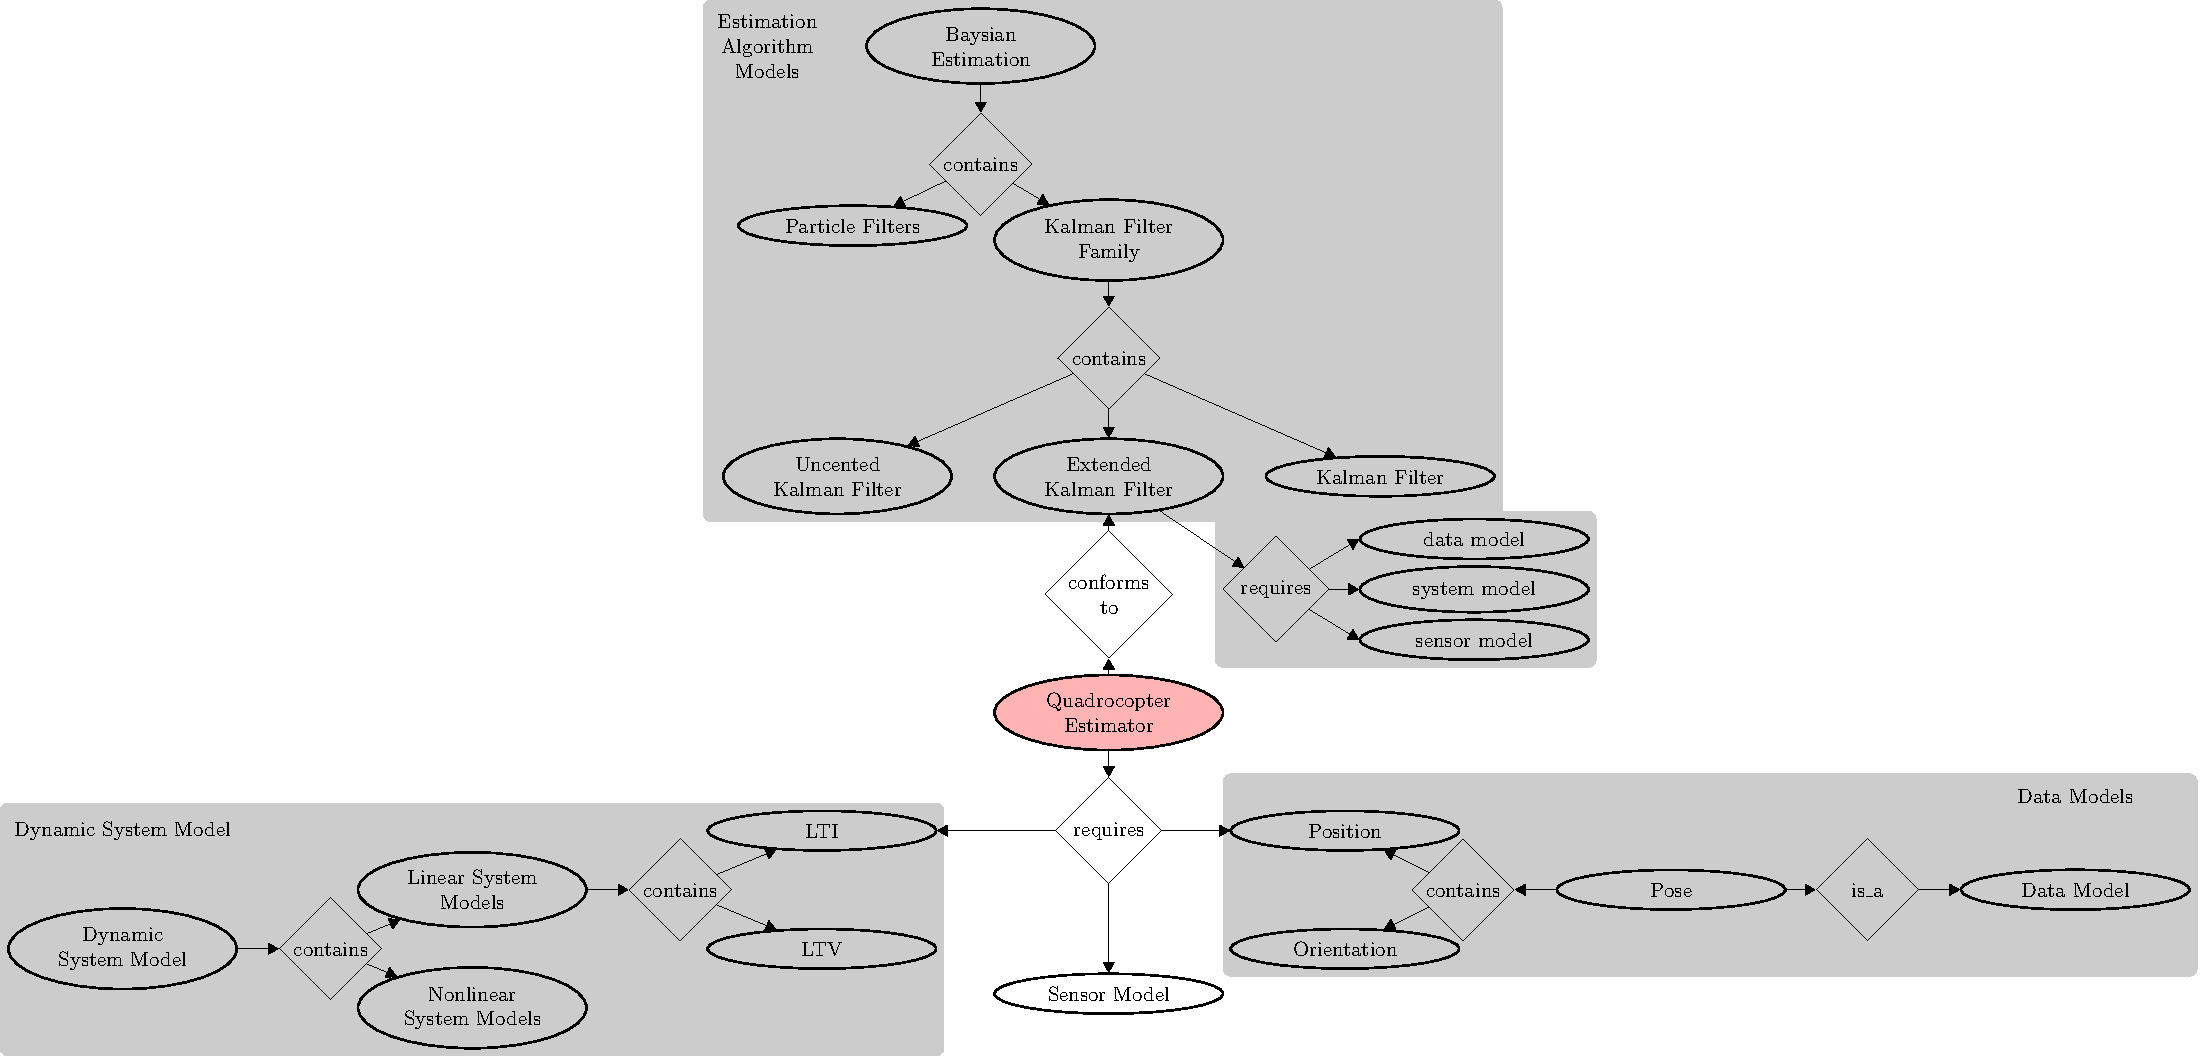
\includegraphics[scale=.6]{ekf_general}

\end{adjustbox}
\end{figure}

 % Chapter 2
\cleardoublepage % Empty page before the start of the next part

%------------------------------------------------

\chapter{Implementation}
\label{ch:implementation}
This chapter gives an introspection of the UBX project and the derived work. There are 3 section: one fore the core libraries, necessary to run nodes, one for the blocks from the official project and one for the blocks designed and implemented in the context of this thesis.

\section{Core UBX library}
This library is composed by the core shared library \texttt{libubx.so} and the Lua scripts and macros necessary to link the component functions together. Please note that since all the UBX functionalities are implemented in C or C++ function, the native Lua interpreter is not capable of linking them; it fact, the LuaJIT interpreter has been used.
\graffito{On \autoref{ch:deploy} Orocos has been used to deploy the node since it supports Lua components, the Orocos Lua interpreter however if currently the native one, for this reason the project itself has been forked and re-linked to the LuaJIT library to allow execution of a MicroBLX node on top of Orocos.}
LuaJIT implements the FFI library which allows calling external C functions and using C data structures from pure Lua code\autocite{bib:luaffi}.\\
The \texttt{Makefile} has been expanded, beyond the compilation directives already present in the official UBX project, it also contains directives to install the core libraries, the scripts and the macro into the system, plus generates a proper configuration file automatically loaded by the \texttt{ubx\_launch} command.

\section{Official UBX Team blocks}
The \texttt{ubx-base} projects contains blocks from the official UBX team; some of those blocks are not used or are re-implemented while others are fundamental for the simulation to work. Moreover it contains the native (basic) data types like \texttt{int}, \texttt{char}, \texttt{long}, \texttt{long long}, \texttt{short}, \texttt{double} and \texttt{float}.
It worths to highlight the presence of two blocks:
\begin{itemize}
	\item \texttt{ptrig}: an s-block that, once properly configured, trigs a list of c-blocks in a timed loop;
	\item \texttt{webif}: this c-block does not need to be triggered nor to be connected: it is able to open a html interface useful to configure, control and monitor the node it is added to.
\end{itemize}

\section{Study-case blocks}
This section describes the blocks designed for the purpose of controlling a quadcopter.

\subsection{Copter controller (\texttt{copter/ctrl\_copter})}
This block implements the control algorithm as explained in \autoref{ch:controlalgorithm} and \autocite{marconi}. It reads the state and the set-point of the vehicle and writes a control action in the form of vectored-thrust control action (i.e. the scalar thrust and the vectored torque the propellers should generate).\\
It is implemented in C++ in order to exploit the capability of the mathematical library Armadillo that greatly simplify operations on vectors and matrices. 

\subsection{Extended predict-only Kalman filter (\texttt{copter/kf\_predict\_copter})}
Models the behavior of the vehicle: reads the estimate of the state and the control action and generate a new estimate of the state (which is usually written back to the same i-block the state was read from).\\
This block is written in C++ and use Armadillo too.

\subsection{Update-only Kalman filter (\texttt{control/kf\_update})}
Fuses the sensor data with the state. Using the notation from Wikipedia\autocite{bib:wiki:kalmann}, the sensor model matrix $ H $ is read from a file specified in the UBX node configuration file while the sensor data covariance matrix $ R $ is computed on-line from the covariance embedded in the sensor data.

\subsection{Fast shm memory access \texttt{control/shm}}
This general-purpose i-block is able to dynamically allocate vectors of arbitrary length of arbitrary data-types in shared memory. Is is used for fast data passing between c-blocks. Data can be accessed by blocks in the same node by properly linking the port connection.\\
Note that, if necessary, multiple shm blocks running on different nodes on the same machine can share the same memory pool, however no synchronization mechanism has been implementer to avoid race condition and therefore it has been chosen to grant write permissions only to the block that allocated the pool while other blocks do only have read access.

\subsection{AHRS+ sensor data acquisition \texttt{control/sensor\_myAHRS}}
This i-block acts as bridge between the node and the physical Hardkernel AHRS+ sensor. It is worth to point out that the official library from the sensor manufacturer can not be used with the \texttt{extern "C"} directive that is instead necessary to run C++ blocks in UBX, so a wrapper has been created.

\subsection{GUI \texttt{copter/copter\_graphic\_dump}}
Even if there is a dump of the state of the controller to the terminal, a graphical output is present too. This is a c-block that when triggered reads the state and the set-point of the vehicle to generate and display a 2-D output. The block use the OpenCV library for the rendering. The block obviously refuse to start out of a graphic environment.\\
The output produced is a view of the vehicle from the top, the size and the center of the environment in wich the copter is moving can be adjusted, the current copter state and set-point is rendered respectively as a red and a green circle with a small tooth to visualize the heading. More detailed information are showed in text format on the top of the screen.

\subsection{Set-point generation \texttt{copter/prim\_trj\_gen}}
The set point of the vehicle is generated by this block from 10 primitives trajectories. The trajectory code is read from a TCP socked, then the primitive trajectory is scaled on the basis of configurable parameters both in time and space and generated as a function of time. The trajectory primitive are, by now, to translate along the 4 cardinal directions, move up and down and rotate by 90 degrees clockwise or anti-clockwise.\\
The code of the primitive is passed via a TCP connection by a GUI application described in \autoref{sec:fakeplanner}, the connection is handled using the ZMQ\cite{bib:ZMQ} library.

\section{Virtual remote controller}
\label{sec:fakeplanner}
 This GUI application act as remote controller for the copter, however it does not directly generates the set-point for the vehicle, which by the way may be unfeasible because of timing constraints, but instead instructs the trajectory generation block about which pre-defined trajectory should generate. This virtual remote controller is named "Fake Planner" because it can (should!) be replaced by a software planner (or supervisor) capable of decision taking.
  % Chapter 2
\cleardoublepage % Empty page before the start of the next part

%------------------------------------------------

\chapter{Simulation}
\label{ch:simulation} 
Since a real copter was not available for testing, 2 proof-of-concept simulation were performed. In the first one the controller has been used with an extended Kalman filter but no sensor has been used: the state of the copter is estimated by mean of the control signal and the model of the copter.

\section{Kalman filter in predict-only mode}

The node core functionality is implemented in the extended Kalman filter and in the controller. The set-point of the copter is computed by the node on the basis of 10 primitives that can be called via a tool that acts as remote controller for the copter, the communication between the node and the controller is realized via a TCP connection.

The controller block \texttt{ctrl} reads the copter state from the block \texttt{state} and the set-point from the block \texttt{setpoint} , than computes and store the control action in \texttt{ctrl\_action}. The Kalman filter block \texttt{kf\_pred\_cptr} in turns reads the state and the control action applied and write the estimate of the state back.

Other blocks are however necessary:
\begin{itemize}
	\item \texttt{ptrig1} is the i-block in charge to call all the c-block of the node (except the graphic dump) in an infinite loop with a period of 1ms;
	\item \texttt{tgj\_gen} is a c-block responsible for generating the current set-point: it receives the trajectory primitive from a tcp connection and computes the actual copter set-point as a function of the time;
	\item \texttt{state} is a i-block that store the state of the copter in virtual memory;
	\item \texttt{setpoint} is a i-block that store the set-point of the copter in virtual memory;
	\item \texttt{ctrl\_action} is a i-block that store the current applied control action in virtual memory;
	\item \texttt{timing} generates a virtual clock allowing to simulate the system beyond the actual computation capabilities of the computer platform.
	\item \texttt{graphic\_dump} opens a gtk 2-D graphic interface showing the position of the copter; a screenshot is reported in \autoref{fig:gfxdump1};
	\item \texttt{ptrig\_graphic} trigs \texttt{graph\_dump} with a period of 10 ms;
\end{itemize}

The configuration file of the node is here reported:
	
	
\begin{lstlisting}[language={[5.0]Lua},]
local bd = require("blockdiagram")

return bd.system {
  imports = {
    "types/stdtypes/stdtypes.so",
    "types/control/control_types.so",
    "blocks/ptrig/ptrig.so",
    "blocks/control/shm.so",
    "blocks/control/dump_ctrl.so",
    "blocks/copter/ctrl_copter.so",
    "blocks/copter/prim_trj_gen.so",
    "blocks/copter/kf_predict_copter.so",
    "blocks/control/dump_state.so",
    "blocks/copter/copter_graphic_dump.so",
    "blocks/control/dump_time_stat.so",
    "blocks/webif/webif.so",
  },

  blocks = {
    { name = "ptrig1" , type = "std_triggers/ptrig" },
    { name = "ptrig_graphic", type = "std_triggers/ptrig" },
    { name = "ctrl_action"  , type = "control/shm" },
    { name = "state"  , type = "control/shm" },
    { name = "setpoint"  , type = "control/shm" },
    { name = "ctrl" , type = "copter/ctrl_copter" },
    { name = "ctrl_dump" , type = "control/dump_ctrl" },
    { name = "state_dump" , type = "control/dump_state" },
    { name = "kf_pred_cptr" , type = "copter/kf_predict_copter" },
    { name = "tgj_gen" , type = "copter/prim_trj_gen" },
    { name = "graph_dump"  , type = "copter/copter_graphic_dump"    },
    { name = "timing"  , type = "control/dump_time_stat"    },
    { name = "webif1"  , type = "webif/webif"    },
  },

  connections = {
    { src="ctrl.ctrl_action" , tgt="ctrl_action" },
    { src="ctrl.ctrl_action" , tgt="ctrl_dump" },
    { src="state" , tgt="ctrl.state" },
    { src="setpoint" , tgt="ctrl.setpoint" },
    { src="kf_pred_cptr.stt_out" , tgt="state" },
    { src="kf_pred_cptr.stt_out" , tgt="state_dump" },
    { src="state" , tgt="kf_pred_cptr.stt_in"  },
    { src="ctrl_action" , tgt="kf_pred_cptr.ctrl_in" },
    { src="tgj_gen.setpoint_out"  , tgt="setpoint" },
    { src="state" , tgt="tgj_gen.state_in" },
    { src="state"      , tgt="graph_dump.state"  },
    { src="setpoint"    , tgt="graph_dump.setpoint"  },
  },

  configurations = {
    {
      name="webif1",
      config = { port="8888" },
    },
		{
			name="kf_pred_cptr" ,
			config = {
				mass		= 1 	,
				J_xx		= 0.01,
				J_yy		= 0.01,
				J_zz		= 0.01,
				dt		= 0.001	,
				process_noise	= 0	,
			},
		},
		{
			name="ctrl_action" ,
			config = {
				shm_name="/ctrl_action" ,
				type_name="struct ControlAction",
			},
		},
		{
			name="setpoint" ,
			config = {
				shm_name="/setpoint" ,
				type_name="struct SetPoint",
			},
		},
		{
			name="state" ,
			config = {
				shm_name="/state" ,
				type_name="struct State",
			},
		},
		{
			name="tgj_gen" ,
			config = {
				dt	= 0.001	;
				zmq_address = "tcp://127.0.0.1:8890"
			},
		},
		{
			name="ctrl" ,
			config = {
				mass		= 1	,
				inertia_xx	= 0.01,
				inertia_yy	= 0.01,
				inertia_zz	= 0.01,
				k1		= 1	,--0.9	,
				l1		= 5	,--5	,	-- i.e. max speed for static set-point
				k2		= 10	,--8	,
				l2		= 10	,--8	,
				kp		= 100	,
				kd		= 10	,
				hysteresis_thr	= 0.01	,
				max_thrust	= 20	,
				max_torque_xx	= 3	,
				max_torque_yy	= 3	,
				max_torque_zz	= 3	,
			},
		},
		{
			name="timing" ,
			config = {
				period		= 60*1000	;
				update_rate	= 0.001		;
			},
		},
		{
			name="ptrig1" ,
			config = {
				period = {sec=0, usec=1000 },
				trig_blocks={
					{ b="#ctrl"		, num_steps=1, measure=0 },
					{ b="#kf_pred_cptr"	, num_steps=1, measure=0 },
					{ b="#tgj_gen"		, num_steps=1, measure=0 },
					{ b="#timing"		, num_steps=1, measure=0 },
				},
			},
		},
		{
			name="graph_dump" ,
			config = {
				zoom = 5 ;
				max_q = 2 ;
			},
		},
		{
			name="ptrig_graphic" ,
			config = {
				period = {sec=0, usec=10000 },
				trig_blocks={
					{ b="#graph_dump"	, num_steps=1, measure=0 },
        },
      },
    },
  },
}
\end{lstlisting}
\subsection{Launching the node}
The node can be lunched by calling the script \texttt{ubx-control/test/04-working\_ctrl/launch.sh}.
This script executes the gtk app \texttt{fake\_planner} specifying with an argument to connect to \texttt{tcp://127.0.0.1:8890} (obviusly the node is configured to listen at the same TCP address and port).\graffito{The name of the remote controller executable is \texttt{fake\_planner} because there may be an actual \emph{mission} planner (or supervisor) controlling the drone instead of a human operator.}.
Then the script launch and deploy the node. Messages from the node are dumped to the terminal but the state of the node can be also checked via a web interface at \texttt{http://127.0.0.1:8888}. \autoref{fig:node04} shows the structure of the node.

\newpage
\begin{figure}
	\centering
	\frame{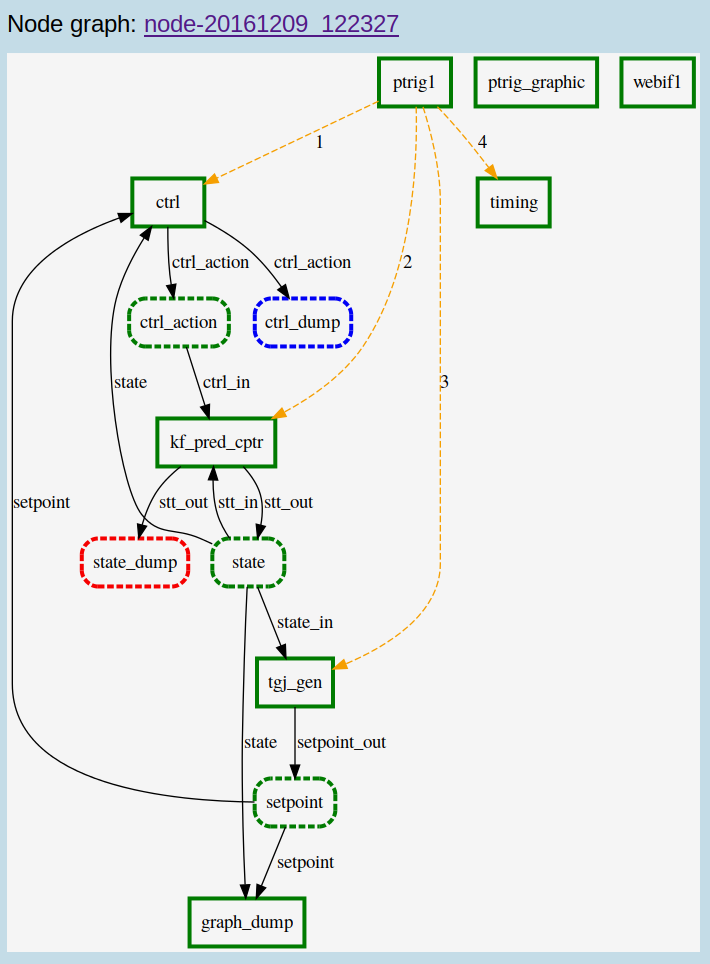
\includegraphics[width=1\textwidth]{node04}}
	\label{fig:node04}
	\caption{The node used for the simulation in predict-only mode}
\end{figure}
\clearpage

\newpage
\begin{figure}
	\centering
	\frame{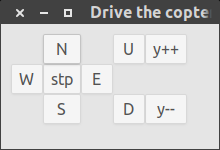
\includegraphics[width=0.3\textwidth]{fakeplanner}}
	\frame{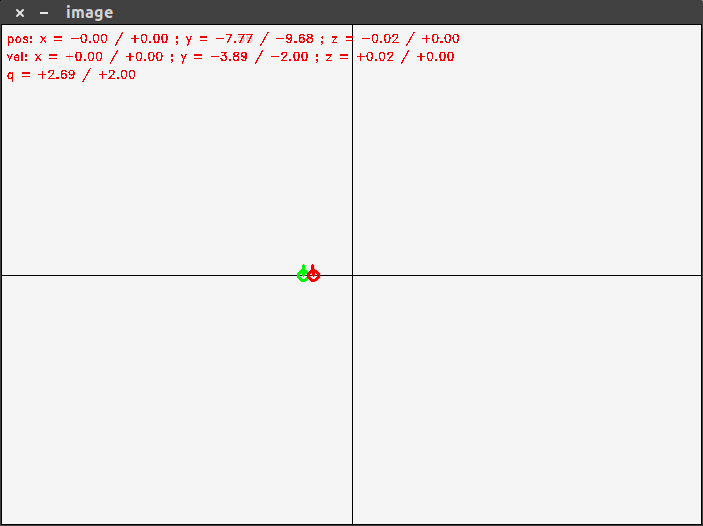
\includegraphics[width=0.8\textwidth]{gfxdump1}}
	\label{fig:gfxdump1}
	\caption{}
\end{figure}
\clearpage


\section{Kalman filter in update-only mode}
The second simulation was performed in a configuration where the Kalman filter is used to update the estimate of the state of the vehicle by reading from an attitude and heading reference system (AHRS) \autocite{bib:wikiahrs}. This application is a proof-of-concept demonstration for sensor fusion and the controller has no role here, the control action is constant (i.e. no feedback) and manually tuned to make the copter hover. The Kalman filter then update the copter attitude with the data from the sensors and accordingly predict the estimate of the position too.\\
The AHRS used is a USB device from Hardkernel \autocite{bib:ahrsproduct}; it embeds a triple axis gyroscope, a triple axis accelerometer and a triple axis magnetometer, plus it embeds an extended Kalman filter (so data if pre-filtered and pre-fused); data can be read via a I2C or UART or USB serial interface. The i-block used to read is a bridge written in C++ named \texttt{sensor\_myAHRS} and can be found in the \texttt{ubx-control} project.

The node can be launched by executing:
\begin{lstlisting}[language=bash]
cd ubx-control/test/06_test_myAHRS/
ubx_launch -c 06.usc -d deploy.udc
\end{lstlisting}
 % Chapter 2
\cleardoublepage % Empty page before the start of the next part

%------------------------------------------------

%\chapter{Deploy}
\label{ch:deploy} 
The simulations showed run with no time constraints while a real use of the software should have hard real-time constraints. The problem of meeting time constrains has multiple solution and can be at least decomposed into two problems:
\begin{itemize}
	\item choose the software component that has to meet the constraint;
	\item how to grantee the time constraint.
\end{itemize}

The first problem can be addressed by simply making the application \emph{stand-alone}, so that the problem becomes trivial. But the s-block previously used does not meet any quality-of-service requirements and should be re-implemented from scratch. The actual solution for this study case has been to deploy the UBX node on Orocos\autocite{bib:orocos}, a well known software framework specifically designed for the deployment of components-oriented hard real-time applications.\\
The second problem has multiple solutions too; for years a common work-around to give the Linux kernel real-time behavior was to apply the \emph{RT-Preempt Patch} \autocite{bib:rtlinux}. A more innovative approach is to rely on cgroups, a Linux Kernel feature which allow processes to be organized into hierarchical groups whose usage of various types of resources can then be limited and monitored\autocite{bib:cgroupsman}. With cgroups, it is possible to assign a pre-defined slice of CPU-time to a process and therefore guarantee the respect of the real-time constraints.

\section{Hard RT requirements}

\section{Orocos}
%git clone git://github.com/orocos-toolchain/rtt.git
%sudo apt install libboost-filesystem-dev
%sudo apt install gcc-4.9
%sudo apt install g++-4.9
%sudo apt install libboost-all-dev 
%sudo apt install libboost-dev 
%sudo apt install libxerces-c-dev
%sudo apt install doxygen

\section{FSM supervisor}
 % Chapter 2
%\cleardoublepage % Empty page before the start of the next part
%\ctparttext{I will describe here the mathematical model of the control algorithm}

%------------------------------------------------
\part{Conclusions}
\chapter{Archived result}
\label{ch:archived} 
This work demonstrates how a component blocks application can be developed in UBX. Obviously, this framework is not as mature as other projects, but introduces some new concepts not present in other environments.\\
The whole application works as expected and can easily be ported to other platform: UBX blocks can be compiled for many CPU architectures: AMD64 and ARM has been tested but it should be possible to compile for microcontrollers too.\\
The time constraints can be easily respected in cheap (but modern) credit-card-sized computer platforms, perhaps a more advanced trigger s-block is necessary.\\
Moreover	 within the context of this thesis some work has been done to deploy a UBX node on the Orocos environment: first, the Ororcos OCL source code has been forked and linked against LuaJIT instead of the native LUA library to allow the usage of the FFI library, the forked repo can be found at:\\
\url{https://github.com/fmr42/ocl}\\
Then the trigger block has been modified to run when triggered by Orocos instead than on a time base. Than the two simulations proposed were launched in this new deploy environment and, as expected, they run as before; the only difference was that the timing for the loop come from the more advance real-time Orocos framework. Also, Linux cgroups where tuned to guarantee the Orocos \emph{hard} real-time constrains.\\
Please note that this last promising result is part of a work still under development, however the Orocos team seamed to appreciate the work done in the fork.
\cleardoublepage % Empty page before the start of the next part

%------------------------------------------------

\chapter{Further work}
\label{ch:further}
\section{UBX limitations}
The UBX framework allows to write blocks with well defined separation of concerns, but does not actually \emph{require} it: a coder could, for example, make a c-block store data in its private memory space, or make a i-block process the data with a computational behavior.\\
Moreover another limitation of UBX is that it still does not support blocks composition, while it should be possible to define sub-nodes to be used as regular blocks.\\
A new library named AB5C is in a very early developing stage and should replace UBX and solve those problematics.

\section{Missing models}
There still is a lack of modeling in this work, also because of the lack of tools to do so. More techniques are under development, especially for data; the goal is to be have (someday) developing frameworks ables to auto-generate the code from models; although there already are tool-chains able to declare (not define!) functions from models, the road to tools able to implement components from mathematical models is still long. By now, the more feasible goal is to have a centralized repository of data models (e.g. positions, rotations, ecc.) to conforms to and at least have data-model transformation tool able to generate "adapter" components to trivially connect components not developed for being connected.\\

\section{Open-source contributions}
As a personal opinion, a large users base is essential to reach high goals and the open source software developing model has proved to work once reached a "critical mass" of developers; as an example, take the ROS project: an environment very similar to UBX that is leading to success thank to a wide adoption in the robotic community.\\
Moreover, universities represent a great source of work force, especially for the complex job of modeling, and should take the initiative in order to tweak a wider (industrial, scientific, recreational, commercial) adoption.


\cleardoublepage % Empty page before the start of the next part
\ctparttext{I will describe here the mathematical model of the control algorithm}


%----------------------------------------------------------------------------------------
%	THESIS CONTENT - APPENDICES
%----------------------------------------------------------------------------------------

%\appendix
%\part{Appendix}
%% Appendix A

\chapter{Quaternions}
\label{ch:app:quaternions} 
Quaternions are a number systems that extends complex numbers introduced by William Rowan Hamilton in 1843. They are commonly represented in the form
\[ q = w + x\mathbf{i} + y\mathbf{j} + z\mathbf{k} \]
where $ \mathbf{i},\ \mathbf{j}\ and\ \mathbf{k} $ are the fundamental quaternion units.
Multiplications between quaternions are non-commutative, with
\begin{table}[]
	\centering
	\caption{My caption}
	\label{my-label}
	\begin{tabular}{|l|l|}
		\hline
		\[ \mathbf{j} x \mathbf{k} = \mathbf{i} \] & \[ \mathbf{j} x \mathbf{k} = \mathbf{i} \] \\ \hline
	\end{tabular}
\end{table}

\[ \mathbf{i} x \mathbf{1} = \mathbf{i} \]
\[ \mathbf{i} x \mathbf{i} = \mathbf{-1} \]
\[ \mathbf{i} x \mathbf{j} = \mathbf{k} \]
\[ \mathbf{i} x \mathbf{k} = \mathbf{-j} \]



\[ \mathbf{k} x \mathbf{1} = \mathbf{i} \]
\[ \mathbf{k} x \mathbf{i} = \mathbf{i} \]
\[ \mathbf{k} x \mathbf{j} = \mathbf{i} \]
\[ \mathbf{k} x \mathbf{k} = \mathbf{i} \]


\section{Rotations}
Normal quaternions are

%\chapter{A new approach to Hard RT in Linux: cgroups}
cgroups are great
%\chapter{Open Source pro and cons}

Open Source rocks

%----------------------------------------------------------------------------------------
%	POST-CONTENT THESIS PAGES
%----------------------------------------------------------------------------------------

\cleardoublepage% Bibliography

\label{app:bibliography} % Reference the bibliography elsewhere with \autoref{app:bibliography}

\manualmark % Work-around to have small caps also here in the headline
\markboth{\spacedlowsmallcaps{\bibname}}{\spacedlowsmallcaps{\bibname}} % Work-around to have small caps also
%\phantomsection
\refstepcounter{dummy}

\addtocontents{toc}{\protect\vspace{\beforebibskip}} % Place the bibliography slightly below the rest of the document content in the table of contents
\addcontentsline{toc}{chapter}{\tocEntry{\bibname}}
\printbibliography

%\cleardoublepage% Declaration

\refstepcounter{dummy}
\pdfbookmark[0]{Declaration}{declaration} % Bookmark name visible in a PDF viewer

\chapter*{Declaration} % Declaration section text

\thispagestyle{empty}

Put your declaration here.
\bigskip
 
\noindent\textit{\myLocation, \myTime}

\smallskip

\begin{flushright}
\begin{tabular}{m{5cm}}
\\ \hline
\centering\myName \\
\end{tabular}
\end{flushright}

%\cleardoublepage% Colophon (a brief description of publication or production notes relevant to the edition)

\pagestyle{empty}

\hfill

\vfill

\pdfbookmark[0]{Colophon}{colophon}

\section*{Colophon}

This document was typeset using the typographical look-and-feel \texttt{classicthesis} developed by Andr\'e Miede. The style was inspired by Robert Bringhurst's seminal book on typography ``\emph{The Elements of Typographic Style}''. \texttt{classicthesis} is available for both \LaTeX\ and \mLyX: 

\begin{center}
\url{https://bitbucket.org/amiede/classicthesis/}
\end{center}

\noindent Happy users of \texttt{classicthesis} usually send a real postcard to the author, a collection of postcards received so far is featured here: 

\begin{center}
\url{http://postcards.miede.de/}
\end{center}
 
\bigskip

\noindent\finalVersionString

%----------------------------------------------------------------------------------------

\end{document}
